\documentclass{beamer}
\usepackage{amsmath}
\usepackage[english]{babel} %set language; note: after changing this, you need to delete all auxiliary files to recompile
\usepackage[utf8]{inputenc} %define file encoding; latin1 is the other often used option
\usepackage{csquotes} % provides context sensitive quotation facilities
\usepackage{graphicx} %allows for inserting figures
\usepackage{booktabs} % for table formatting without vertical lines
\usepackage{textcomp} % allow for example using the Euro sign with \texteuro
\usepackage{stackengine}
\usepackage{wasysym}
\usepackage{tikzsymbols}
\usepackage{textcomp}
\newcommand{\bubblethis}[2]{
        \tikz[remember picture,baseline]{\node[anchor=base,inner sep=0,outer sep=0]%
        (#1) {\underline{#1}};\node[overlay,cloud callout,callout relative pointer={(0.2cm,-0.7cm)},%
        aspect=2.5,fill=yellow!90] at ($(#1.north)+(-0.5cm,1.6cm)$) {#2};}%
    }%
\tikzset{face/.style={shape=circle,minimum size=4ex,shading=radial,outer sep=0pt,
        inner color=white!50!yellow,outer color= yellow!70!orange}}
%% Some commands to make the code easier
\newcommand{\emoticon}[1][]{%
  \node[face,#1] (emoticon) {};
  %% The eyes are fixed.
  \draw[fill=white] (-1ex,0ex) ..controls (-0.5ex,0.2ex)and(0.5ex,0.2ex)..
        (1ex,0.0ex) ..controls ( 1.5ex,1.5ex)and( 0.2ex,1.7ex)..
        (0ex,0.4ex) ..controls (-0.2ex,1.7ex)and(-1.5ex,1.5ex)..
        (-1ex,0ex)--cycle;}
\newcommand{\pupils}{
  %% standard pupils
  \fill[shift={(0.5ex,0.5ex)},rotate=80] 
       (0,0) ellipse (0.3ex and 0.15ex);
  \fill[shift={(-0.5ex,0.5ex)},rotate=100] 
       (0,0) ellipse (0.3ex and 0.15ex);}

\newcommand{\emoticonname}[1]{
  \node[below=1ex of emoticon,font=\footnotesize,
        minimum width=4cm]{#1};}
\usepackage{scalerel}
\usetikzlibrary{positioning}
\usepackage{xcolor,amssymb}
\newcommand\dangersignb[1][2ex]{%
  \scaleto{\stackengine{0.3pt}{\scalebox{1.1}[.9]{%
  \color{red}$\blacktriangle$}}{\tiny\bfseries !}{O}{c}{F}{F}{L}}{#1}%
}
\newcommand\dangersignw[1][2ex]{%
  \scaleto{\stackengine{0.3pt}{\scalebox{1.1}[.9]{%
  \color{red}$\blacktriangle$}}{\color{white}\tiny\bfseries !}{O}{c}{F}{F}{L}}{#1}%
}
\usepackage{fontawesome} % Social Icons
\usepackage{epstopdf} % allow embedding eps-figures
\usepackage{tikz} % allows drawing figures
\usepackage{amsmath,amssymb,amsthm} %advanced math facilities
\usepackage{lmodern} %uses font that support italic and bold at the same time
\usepackage{hyperref}
\usepackage{tikz}

\usepackage{tcolorbox}

\usefonttheme[onlymath]{serif} %set math font to serif ones

\definecolor{beamerblue}{rgb}{0.2,0.2,0.7} %define beamerblue color for later use

%%% defines highlight command to set text blue
\newcommand{\highlight}[1]{{\color{blue}{#1}}}


%%%%%%% commands defining backup slides so that frame numbering is correct

\newcommand{\backupbegin}{
   \newcounter{framenumberappendix}
   \setcounter{framenumberappendix}{\value{framenumber}}
}
\newcommand{\backupend}{
   \addtocounter{framenumberappendix}{-\value{framenumber}}
   \addtocounter{framenumber}{\value{framenumberappendix}}
}

%%%% end of defining backup slides

%Specify figure caption, see also http://tex.stackexchange.com/questions/155738/caption-package-not-working-with-beamer
\setbeamertemplate{caption}{\insertcaption} %redefines caption to remove label "Figure".
%\setbeamerfont{caption}{size=\scriptsize,shape=\itshape,series=\bfseries} %sets figure  caption bold and italic and makes it smaller


\usetheme{Boadilla}

% --------------------
% Overall information
% --------------------

\title[Economía I]{Economía I \vspace{4mm}
\\ Magistral 14: El rol del mercado}
\date{}
\author[Ertola Navajas y Fariña]{Ertola Navajas y Fariña}
\vspace{0.4cm}
\institute[]{Universidad de San Andrés} 

\begin{document}

\begin{frame}
\titlepage
\centering
\includegraphics[scale=0.2]{../Figures/logoUDESA.jpg} 
\end{frame}

\begin{frame}{Mercados vs Planificación}
    
    \begin{itemize}
        \item ¿Cuál era el problema económico?
        \item ¿Se acuerdan el ejemplo de los tazones? 
        \vspace{1mm}
        \item El ejemplo nos permite ilustrar los problemas de la asignación considerando distintos mecanismos: asignación de mercado versus planificación
        \vspace{1mm}
        \item ¡Y también comparar estos mecanismos! 
    \end{itemize}
\end{frame}

\begin{frame}{Algunos problemas de la planificación}
    \begin{itemize}
        \item Es muy intensivo en información requerida (necesita conocer perfectamente preferencias y costos)  \vspace{1mm}
            \begin{itemize} [l{-}] 
                \item  Ejemplo de Cheqoslovaquia
            \end{itemize}
            \vspace{1mm}
        \item Genera incentivos incorrectos  \vspace{1mm}
            \begin{itemize} [l{-}]
                \item Ejemplo de la China Maoísta
            \end{itemize}
            \vspace{1mm}
        \item Resulta inconsistente con las libertades políticas  ''
            \begin{itemize} [l{-}]
                \item ``El camino a la servidumbre'' de Hayek     
            \end{itemize}
            \begin{itemize} [l{-}]
                \item Concepto de ``Libertad como desarrollo'' de Amartya Sen
            \end{itemize}
    \end{itemize}
\end{frame}

\begin{frame}{La peli recomendada}
    \centering  
    \href{https://www.youtube.com/watch?v=u5hzmwGW4Ac}{\includegraphics[scale=0.95]{../Figures/Goodbyelenin.png}}  
\end{frame}

\begin{frame}{La mano invisible de Adam Smith}
    \begin{quote}
    “No es la benevolencia del carnicero, cervecero o panadero de donde obtendremos nuestra cena, sino de su preocupación por sus propios intereses”
\end{quote}
\end{frame}

\begin{frame}{Eficiencia de mercado}

     \begin{figure}[H]{\textwidth}
         \centering
         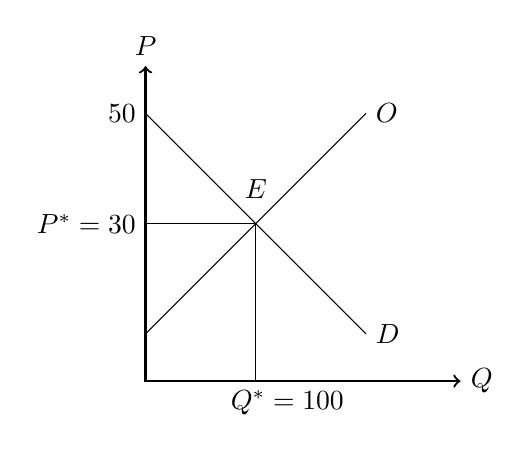
\begin{tikzpicture}[scale=0.4]
\draw[thick,<->] (0,10) node[above]{$P$}--(0,0)--(10,0) node[right]{$Q$};
%\node [below left] at (0,0) {$0$};
\node [below] at (4.5,0) {$Q^*=100$};
\node [above] at (7/2,5.5) {$E$};
\node [left] at (0,5) {$P^*=30$};
%\node [left] at (0,6.85) {$40$};
\node [left] at (0,8.5) {$50$};
%\node [below] at (1.75,0) {50};
%\draw[semithick, red](1.75,5)--(1.75,6.85);
%\draw[thick,gray, dashed](1.75,0)--(1.75,6.85)--(0,6.85);
\draw[](0,5)--(7/2,5)--(7/2,0);
\draw[black, domain=0:7] plot (\x, {8.5-\x}) node[right] {$D$};
\draw[black, domain=0:7] plot (\x, {1.5+\x}) node[right] {$O$};
\end{tikzpicture}
     \end{figure}
El mercado produce la cantidad óptima del bien: solo se produce si vale más que lo que cuesta producirlo
\end{frame}

\begin{frame}{Eficiencia de mercado II}

    \begin{figure}{\textwidth}
         \centering
         \tikzset{every picture/.style={line width=0.75pt}} %set default line width to 0.75pt        
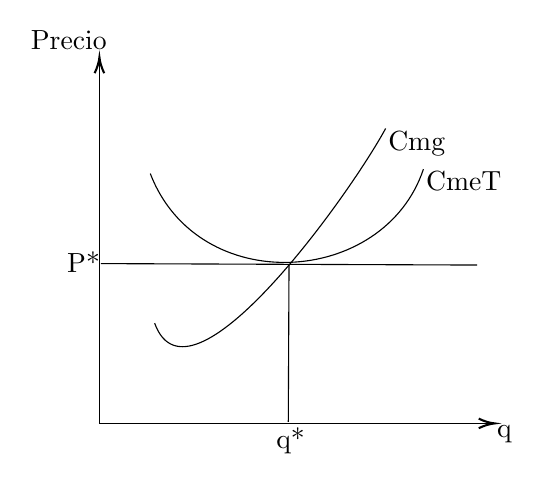
\begin{tikzpicture}[x=0.75pt,y=0.75pt,yscale=-0.7,xscale=0.7] 
%uncomment if require: \path (0,1657); %set diagram left start at 0, and has height of 1657

%Straight Lines [id:da6123979361342768] 
\draw    (74,298) -- (344,298) ;
\draw [shift={(346,298)}, rotate = 180] [color={rgb, 255:red, 0; green, 0; blue, 0 }  ][line width=0.75]    (10.93,-3.29) .. controls (6.95,-1.4) and (3.31,-0.3) .. (0,0) .. controls (3.31,0.3) and (6.95,1.4) .. (10.93,3.29)   ;
%Straight Lines [id:da5131707791527922] 
\draw    (74,298) -- (74,48) ;
\draw [shift={(74,46)}, rotate = 450] [color={rgb, 255:red, 0; green, 0; blue, 0 }  ][line width=0.75]    (10.93,-3.29) .. controls (6.95,-1.4) and (3.31,-0.3) .. (0,0) .. controls (3.31,0.3) and (6.95,1.4) .. (10.93,3.29)   ;
%Straight Lines [id:da6346804843028921] 
\draw    (75,188) -- (334,189) ;
%Curve Lines [id:da697350144213293] 
\draw    (109,126) .. controls (142,212) and (270,204) .. (297,123) ;
%Curve Lines [id:da9799910224345574] 
\draw    (112,229) .. controls (136,295) and (246,141) .. (271,95) ;
%Straight Lines [id:da5845279516726063] 
\draw    (204.5,188.5) -- (204,297) ;

% Text Node
\draw (25,26) node [anchor=north west][inner sep=0.75pt]   [align=left] {Precio};
% Text Node
\draw (346,298) node [anchor=north west][inner sep=0.75pt]   [align=left] {q};
% Text Node
\draw (297,123) node [anchor=north west][inner sep=0.75pt]   [align=left] {CmeT};
% Text Node
\draw (271,95) node [anchor=north west][inner sep=0.75pt]   [align=left] {Cmg};
% Text Node
\draw (50,178) node [anchor=north west][inner sep=0.75pt]   [align=left] {P*};
% Text Node
\draw (194,299) node [anchor=north west][inner sep=0.75pt]   [align=left] {q*};

\end{tikzpicture}
     \end{figure}

En el largo plazo, el mercado produce cada bien al MENOR costo medio posible dada la tecnología
\end{frame}

\begin{frame}{Distorsiones al equilibrio de mercado}
    \begin{itemize}
        \item En muchas ocasiones el mercado no funciona tan perfectamente
        \vspace{1mm}
        \item Hay dos tipos de desvíos
        \begin{itemize}
            \item Los creados por el hombre
            \item Los que se imponen por características de la realidad
        \end{itemize}
    \end{itemize}
\end{frame}


\begin{frame}{Distorsiones al equilibrio de mercado}
    \begin{itemize}
        \item Creadas por el hombre:
        \begin{itemize}
            \item Monopolios artificiales (farmacias, escribanos, low cost)
             \vspace{1mm}
            \item Impuestos
             \vspace{1mm}
            \item Precios máximos o mínimos (cepo)
             \vspace{1mm}
            \item Regulación (ley de alquileres)
        \end{itemize}
    \end{itemize}
\end{frame}

\begin{frame}{Distorsiones al equilibrio de mercado}
    \begin{itemize}
        \item Por las características de la realidad \vspace{1mm}
        \begin{itemize}
            \item Monopolios naturales (red eléctrica, agua, gas)   
             \vspace{1mm}
            \item Externalidades
             \vspace{1mm}
            \item Bienes públicos
            \vspace{1mm}
            \item Problemas de información
            \begin{itemize}
                \item Atributos ocultos (selección adversa)
                 \vspace{1mm}
                \item Acciones ocultas (moral hazard)
            \end{itemize}        
        \end{itemize}
    \end{itemize}
\end{frame}

%\begin{frame}{La introducción de un impuesto}

%\begin{figure} [H]
%\caption{¡Genera un costo de eficiencia!}
%   \centering
%\begin{tikzpicture}[scale=0.6]
%\draw[very thick,<->] (0,10) node[above]{$P$}--(0,0)--(10,0) node[right]{$Q$};
%\draw[semithick](1,2)--(8,9) node[right]{$O'$};
%\draw[semithick](2,1)--(9,8) node[right]{$O$};
%\draw[semithick](1,9)--(9,1) node[right]{$D$};
%\path[pattern=horizontal lines,pattern color=black] (4.5,3.6)--(4.5,5.5)--(5.4,4.5);
%\draw[semithick,dashed,gray](0,5.5)--(4.5,5.5)--(4.5,0);
%\draw[semithick,dashed, gray](0,3.6)--(4.5,3.6);
%\node [right] at (7,5) {\scriptsize Triángulo de};
%\node [right] at (7.25,4.5) {\scriptsize Harberger};
%\draw[semithick, <-] (5.3,4.2)..controls (5.8,3.8) and (6.8,3.8)..(7.5,4.2);
%\draw[semithick,dashed,gray](0,4.5)--(5.5,4.5)--(5.5,0);
%\node[below] at(5.5,0) {\footnotesize $Q*$};
%\node[below] at(4.5,0) {\footnotesize $Q'$};
%\node[left] at(0,4.5) {\footnotesize $P*$};
%\node[left] at(0,5.5) {\footnotesize $P'_C$};
%\node[left] at(0,3.6) {\footnotesize $P'_P$};
%\end{tikzpicture}
%\label{fig:20.2}
%\end{figure}

%\end{frame}


\begin{frame}
\frametitle{El impacto de los impuestos}
\begin{itemize}
    \item ¿Qué es un impuesto?
    \begin{itemize}
        \item Es un tributo generalmente establecido por el Estado 
        - para financiar sus gastos
        - para ‘guiar’ el comportamiento (por ejemplo en el caso de externalidades)
    \end{itemize}
    \item Existen diversos tipos:
    \begin{itemize}
        \item Al consumo, al trabajo, al ingreso, a la propiedad, etc.
    \end{itemize}
    \item Un impuesto aumentará el precio que los consumidores pagan sobre un bien...
    \item La elasticidad precio de la demanda tendrá influencia sobre el efecto del impuesto
\end{itemize}
\end{frame}

\begin{frame}
\frametitle{Impuestos y eficiencia}
\begin{itemize}
    \item La introducción de impuestos aleja la economía del equilibrio competitivo
    \begin{itemize}
        \item Los impuestos sobre oferentes/consumidores desplazan la curva de oferta/demanda porque el precio es más alto para cada cantidad
        \item Al recaudar impuestos el Estado genera una pérdida de peso muerto
    \end{itemize}
    \item La recaudación se extrae del excedente de consumidores y productores
    \begin{itemize}
        \item La incidencia del impuesto depende de la elasticidad relativa de consumidores y productores
        \item El grupo menos elástico lleva más de la carga fiscal
    \end{itemize}
\end{itemize}
\end{frame}

\begin{frame}
\frametitle{Impacto de un impuesto a los vendedores}
\includegraphics[scale=0.6]{../Figures/Tema_07.29_impuesto1.jpg}
\end{frame}

\begin{frame}
\frametitle{Impacto de un impuesto a los vendedores}
\includegraphics[scale=0.6]{../Figures/Tema_07.30_impuesto2.jpg}
\end{frame}

\begin{frame}
\frametitle{Impacto de los impuestos}
\begin{itemize}
    \item ¿Cuánto va a cambiar los impuestos el comportamiento de los individuos?
    \begin{itemize}
        \item ¿Qué tan grande va a ser la pérdida de peso muerto? \\
        - ¿Porqué es relevante conocer la elasticidad de demanda? \\
        - ¿Qué tipo de productos tienen demanda inelástica?
    \end{itemize}
    \item ¿Qué hace el gobierno con los recursos que recauda?
    \item A veces el gobierno quiere cambiar el comportamiento
\end{itemize}
\end{frame}

\begin{frame}
\frametitle{Impuestos y elasticidad}
\begin{itemize}
    \item Un impuesto puede reducir mucho las ventas si su demanda es altamente elástica
    \begin{itemize}
        \item ¡Y eso puede ser lo que el gobierno intenta hacer! \\
        - P.ej., impuestos sobre bienes ‘malos’ para la sociedad como el tabaco o el alcohol o por contaminar
    \end{itemize}
    \item Pero si un impuesto causa una importante caída en las ventas, también reduce los ingresos del impuesto
    \item Si un gobierno que desea aumentar los ingresos a partir del impuesto, debería elegir gravar productos con demanda inelástica
    \begin{itemize}
        \item ¿Qué tipo de productos pueden tener una demanda de estas características?
    \end{itemize}
\end{itemize}
\end{frame}

\begin{frame}
\frametitle{Veamos un ejemplo}
\begin{itemize}
    \item La demanda es Q = 7000 - 40 P 
    \item La oferta Q = 100 P
    \item El gobierno coloca un impuesto de \$10
\end{itemize}
\end{frame}

\begin{frame}
\frametitle{Minimizando la distorsión}
\begin{itemize}
    \item Elasticidad y pérdida de eficiencia 
    \item Otros criterios: redistribución, salud
    \item Esquemas distorsivos: Nafta y Monotributo + TdF
    \item Impuestos que distorsionan el procesos productivo: IVA vs IIBB
    \item Impuestos directos e indirectos
\end{itemize}
\end{frame}

\begin{frame}{Los impuestos en Argentina}
\centering
 \includegraphics[scale=0.6]{../Figures/Impositiva.png}   
\end{frame}

\begin{frame}{Los impuestos en Argentina}
\centering
 \includegraphics[scale=0.6]{../Figures/Impositiva II.png}   
\end{frame}

\begin{frame}{Minimizando las distorsiones}

\begin{figure} [H]
\caption{Impuestos con producto totalmente inelástico}
    \centering
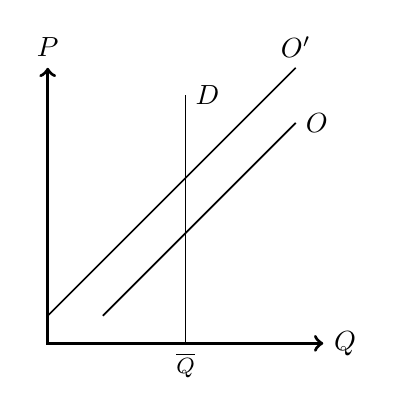
\begin{tikzpicture}[scale=0.35]
\draw[ very thick,<->] (0,10) node[above]{$P$}--(0,0)--(10,0) node[right]{$Q$};
%\node [below left] at (0,0) {$0$};
\draw[semithick](0,1)--(9,10) node[above]{$O'$};
\draw[semithick](2,1)--(9,8) node[right]{$O$};
\draw[semithick](5,0)--(5,9) node[right]{$D$};
\node[below] at(5,0) {\footnotesize $\overline{Q}$};
\end{tikzpicture}
\label{fig:20.1}
\end{figure} 

\begin{itemize}
    \item Queremos grabar los bienes más inelásticos
    \item Si todos los bienes tienen la misma elasticidad entonces tendran la misma tasa
\end{itemize}
\end{frame}

\begin{frame}
\frametitle{Y si tengo un subsidio...}

\end{frame}

\end{document}
